% !TeX spellcheck = hu_HU
\documentclass[12pt,a4paper]{article}
\usepackage[utf8]{inputenc}
\usepackage{cmap}
\usepackage[T1]{fontenc}
\usepackage[magyar]{babel}
\usepackage{amsmath}
\usepackage{amsfonts}
\usepackage{amssymb}
\usepackage{graphicx}

\usepackage{outlines}
\usepackage{hyperref}

\hyphenpenalty=10000

\newcommand{\gto}{\Rightarrow_G}
%\newcommand{\gto}{{\implies \atop G}}
\newcommand{\gtos}{\Rightarrow_G^*}
\newcommand{\ato}{\Rightarrow_A}
\newcommand{\atos}{\Rightarrow_A^*}

\begin{document}

\begin{center}
	\huge
	Formális nyelvek és fordítóprogramok alapjai\\
	\vspace{1mm}
	\LARGE
	Formális nyelvek témakör jegyzete\\
	\vspace{5mm}
	\large
	Készült Nagy Sára előadásai\\
	és Dévai Gergely gyakorlatai alapján\\
	\vspace{5mm}
	Sárközi Gergő, 2021-22-2. félév\\
	Nincsen lektorálva!
\end{center}

\tableofcontents

\pagebreak

\section{Előadás 1: Alapfogalmak és jelölések}

\begin{outline}
	\1 Két halmaz akkor egyenlő, ha egymásnak részhalmazai.
	\1 Ábécé: jelek egy nem üres véges halmaza, jele: $V$
	\1 Betű: ábécé elemei ($a \in V$)
	\1 Szó: $V$ feletti szó a $V$ ábécé elemeinek véges sorozata (szó=sztring)
		\2 $u$ szó hossza: $\ell(u)$ \; ($0 \le \ell(u) < \infty$)
		\2 üres szó: $\epsilon$ \; ($\ell(\epsilon) = 0$)
	\1 $V^*$: $V$ ábécé feletti szavak halmaza
		\2 $\epsilon \in V^*$, de $V^+ = V \setminus \{\epsilon\}$
	\1 Nyelv, formális nyelv: $V^*$ egy bizonyos részhalmaza, jele: $L$
		\2 Létezik véges és végtelen nyelv
		\2 Üres szót tartalmazó nyelv: $\{\epsilon\}$
		\2 Üres nyelv: $\emptyset$
	\1 Nyelvosztály, nyelvcsalád: nyelvek valamely halmaza
	\1 Lexikografikus rendezés: először hosszúság szerint, utána ábécé szerint
		\2 Véges és végtelen nyelveket is el lehet kezdeni felsorolni így
\end{outline}

\subsection{Szavak műveletei}

\begin{outline}
	\1 Konkatenáció: szavak egymás után leírása
		\2 Nincs műveleti jel: csak egymás után leírjuk a szimbólumokat
		\2 Egységelem: $\epsilon$
		\2 Asszociatív: $(uv)w=u(vw)$ \; ($u,v,w \in V^*$)
		\2 $V^*$ zárt a konkatenáció műveletre
	\1 Hatványozás: szó önmagával vett $n$-szeres konkatenációja
		\2 $u^0=\epsilon$, $u^1=u$ és ha $n \ge 1$: $u^n=u^{n-1}u$
	\1 Szó megfordítása: betűk hátulról előre olvasva, jele: $u^{-1}$
\end{outline}

\subsubsection{Részszó, szó prefix, szó szuffix}

\begin{outline}
	\1 Részszó: $v$ az $u$ részszava, ha létezik $x,y$ szó, hogy $u=xvy$
	\1 Szó prefixe: $v$ az $u$ prefixe, ha létezik $w$ szó, hogy $u=vw$
	\1 Szó szuffixe: $v$ az $u$ szuffixe, ha létezik $w$ szó, hogy $u=wv$
	\1 "Valódi" jelentése: a teljes szó és az üres szó nem számít bele
		\2 Azaz $v \ne \epsilon$ és $v \ne u$
\end{outline}

\subsection{Nyelvek műveletei}

\begin{outline}
	\1 Reguláris műveletek: unió, konkatenáció, lezárás
	\1 Két nyelv uniója: ha $L_1,L_2 \subseteq V^*$: $L_1 \cup L_2 = \{u \in V^* \;|\; u \in L_1 \lor u \in L_2\}$
		\2 Ha nem mindkettő $V^*$ feletti: ábécé unióját is vesszük
		\2 Kommutatív, asszociatív, egységelemes ($\emptyset$)
	\1 Két nyelv metszete: $L_1 \cap L_2 = \{u \in V^* \;|\; u \in L_1 \wedge u \in L_2\}$
	\1 Egy nyelv komplementere egy ábécére vonatkozóan: $\overline{L} = V^* \setminus L$
	\1 Egy nyelv tükörképe: $L^{-1} = \{u \in V^* \;|\; u^{-1} \in L \}$
	\1 Két nyelv konkatenációja: $L_1 L_2 = \{uv \;|\; u \in L_1 \wedge v \in L_2\}$
		\2 Gyakorlatilag szorzat
		\2 Asszociatív, egységelemes ($\{\epsilon\}$)
		\2 Van nullelem: $\emptyset L = \emptyset = L \emptyset$
	\1 Nyelv hatványozása: ismételt konkatenáció önmagával
		\2 $L^0 = \{\epsilon\}$, $L^1=L$ és ha $n \ge 1$: $L^n=L^{n-1}L$
		\2 $\emptyset^0 = \{\epsilon\}$ \; ($\emptyset$ minden más hatványa önmaga)
	\1 Nyelv lezártja (iteráltja): $L^*=L^0 \cup L^1 \cup L^2 \cup ...$
		\2 $L^+ = \bigcup\limits_{i \ge 1} L^i$ \; ($\epsilon \in L^+ \Leftrightarrow \epsilon \in L$)
\end{outline}

\pagebreak

\section{Előadás 2: grammatika}

\begin{outline}
	\1 Nyelv megadható szabályrendszerrel (de nem mindegyik)
	\1 Grammatika (nyelvtan): $G=(N,T,P,S)$
		\2 $N$: nemterminális ábécé (szimbólumok, nagybetűsek)
		\2 $T$: terminálisok ábécéje (bemeneti szöveg ábécéje, kisbetűsek)
		\2 $P$: átírási szabályok véges halmaza
		\2 $S$: kezdőszimbólum ($S \in N$)
		\2 $N$ és $T$ diszjunkt halmazok
	\1 Átírási szabályok 
		\2 $p \to q$ alakúak, ahol $p \in (N \cup T)^*N(N \cup T)^*$ és $q \in (N \cup T)^*$
			\3 Bal oldal tartalmaz min. 1 nemterminális szimbólumot
			\3 Jobb oldal lehet üres
		\2 Mondatforma: $(N \cup T)^*$ (vegyes karakterek)
			\3 Ha nem vegyes, akkor mondatforma is, de szó is
\end{outline}

\subsection{Levezetés}

\begin{outline}
	\1 $v$ közvetlen levezethető $u$-ból ($u \gto v$), ha: \;\; ($u,v \in (N \cup T)^*$)
		\2 Létezik $u_1,u_2 \in (N \cup T)^*$ és $x \to y \in P$
		\2 Hogy: $u=u_1 \, x \, u_2$ és $v=u_1 \, y \, u_2$
	\1 $v$ közvetetten levezethető $u$-ból ($u \gtos v$), ha: \;\; ($u,v \in (N \cup T)^*$)
		\2 Létezik $k \in \mathbb{N}$ és $x_0,...,x_k \in (N \cup T)^*$
		\2 Hogy: $u=x_0$ és $v = x_k$ és $\forall i \in [0,k-1]: x_i \gto x_{i+1}$
	\1 Grammatika által generált nyelv
		\2 Minden olyan szó, ami (közvetetten) levezethető $S$-ből
		\2 $L(G) = \{u \in T^* \; | \; S \gtos u \}$
	\1 Példa: $G=(\{S,A,B\}, \{a,b\}, P, S)$
		\2 $P=\{S \to ASB,\; S \to AB,\; AB \to BA,\; A \to a,\; B \to b \}$
		\2 $L(G) = \{u \in \{a,b\}* \;|\; \ell_a(u) = \ell_b(u) \ge 1 \}$
		\2 Példa: $S \gtos A^nB^n \gtos A^{n-1}BAB^{n-1} \gtos BA^nB^{n-1} \gtos ba^nb^{n-1}$
\end{outline}

\pagebreak

\subsection{Chomsky féle grammatika típusok}

\begin{outline}
	\1 A $G=(N,T,P,S)$ grammatikát $P$ alapján lehet osztályozni
	\1 $i=0$ típus: nincs korlátozás (azaz ennyi: grammatikával megadható)
	\1 $i=1$ típus, környezetfüggő: $P$ minden szabálya $u_1Au_2 \to u_1vu_2$ alakú,\\
	ahol $u_1,u_2,v \in (N \cup T)^*$, $A \in N$ és $v \ne \epsilon$,\\
	kivéve az $S \to \epsilon$ alakú szabály (Korlátozott $\epsilon$ szabály, KES), de ekkor $S$ nem fordul elő egyetlen szabály jobboldalán sem.
	\1 $i=2$ típus, környezetfüggetlen: $P$ minden szabálya $A \to v$ alakú,\\
	ahol $A \in N, v \in (N \cup T)^*$
	\1 $i=3$ típus, reguláris grammatika: $P$ minden szabálya\\
	vagy $A \to uB$ vagy $A \to u$ alakú, ahol $A,B \in N$ és $u \in T^*$
	\1 Jelölje $\mathcal{G}_i$ az $i$ típusú grammatikák halmazát
		\2 $\mathcal{G}_i \subseteq \mathcal{G}_0$ ahol $i \in \{1,2,3\}$
		\2 $\mathcal{G}_3 \subseteq \mathcal{G}_2 \not \subseteq \mathcal{G}_1 \subseteq \mathcal{G}_0$
			\3 Hiányzó tartalmazás oka: $\epsilon$-nal kapcsolatos kikötések
			\3 Epszilon mentes grammatika esetén van tartalmazás ott is
	\1 Alábbi táblázat sorai egymásba alakítható grammatikák
\end{outline}

\begin{figure}[h!]
	\centering
	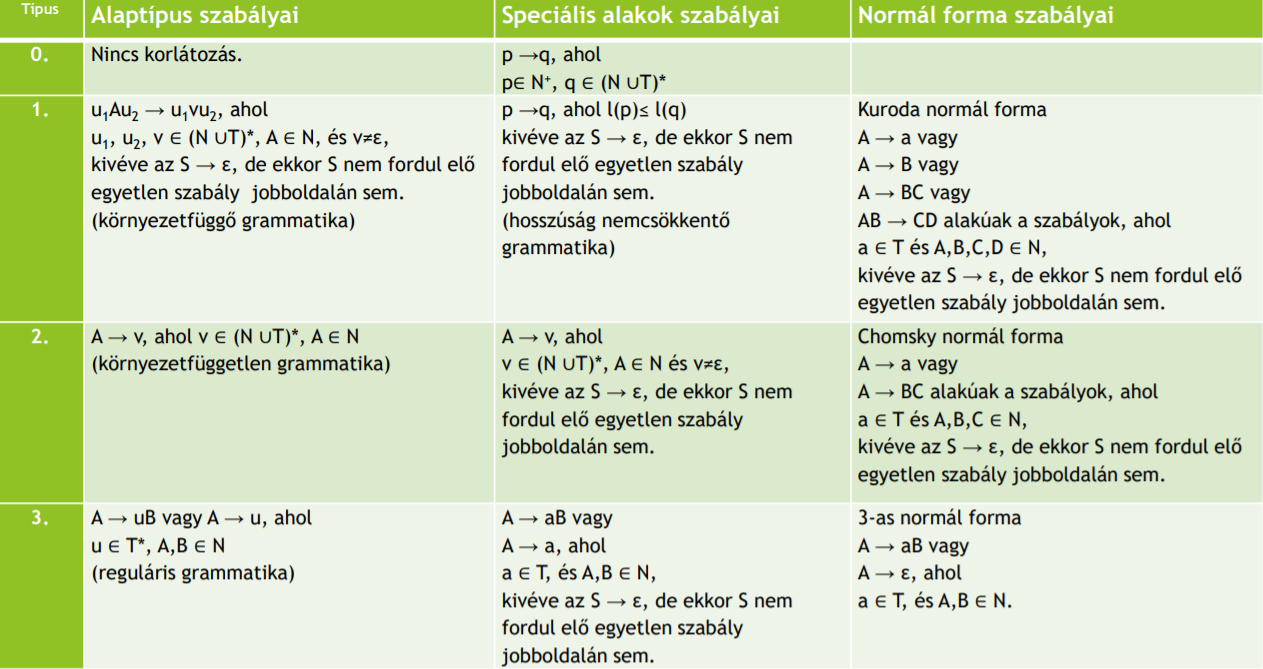
\includegraphics[width=1\linewidth]{grammatika-típusok}
\end{figure}

\pagebreak

\subsubsection{Grammatika típusuk implementálási igényei}

\begin{outline}
	\1 3-as típusú grammatika verem nélkül is implementálható
	\1 2-es nyelvcsaládhoz már kell 1 verem
	\1 Két veremmel már bármi lehetséges (0-as nyelvcsalád)
\end{outline}

\subsection{Példa grammatika típusára}

\begin{outline}
	\1 Kérdés $G=(\{S',S,A,B\}, \{a,b\}, P, S')$ grammatika típusa
	\1 $P = \begin{cases}
	S' \to \epsilon & \text{KES}\\
	S' \to S & \text{0,1,2,3 típusú szabály}\\
	S \to ASB & \text{0,1,2 típusú szabály}\\
	S \to AB & \text{0,1,2 típusú szabály}\\
	AB \to BA & \text{0 típusú szabály (TODO miért nem 1?)}\\
	A \to a & \text{0,1,2,3 típusú szabály}\\
	B \to b & \text{0,1,2,3 típusú szabály}
	\end{cases}$
	\1 Tehát $G$ grammatika 0-s típusú, $G_1 \in \mathcal{G}_0$
\end{outline}

\subsection{Nyelvtanok ekvivalenciája}

\begin{outline}
	\1 $G_1$ és $G_2$ ekvivalensek, ha $L(G_1) = L(G_2)$
	\1 Gyengén ekvivalensek, ha $L(G_1) \setminus \{\epsilon\} = L(G_2) \setminus \{\epsilon\}$
\end{outline}

\subsection{Nyelvek típusai}

\begin{outline}
	\1 Egy $L$ nyelv $i$ típusú, ha $\exists$ $i$-típusú grammatika, ami generálja
	\1 Nyelvcsalád: $\mathcal{L}_i$ jelöli az $i$-típusú nyelvek halmazát
	\1 Chomsky féle hierarchia: $\mathcal{L}_3 \subset \mathcal{L}_2 \subset \mathcal{L}_1 \subset \mathcal{L}_0$
\end{outline}

\subsection{Kényelmi jelölés}

\begin{outline}
	\1 $S \to A \;|\; B$ jelentése: két szabály, $S \to A$ és $S \to B$
\end{outline}

\subsection{Bizonyítások}

\begin{outline}
	\1 Indukcióval
\end{outline}

\pagebreak

\section{Előadás 3: reguláris műveletek és nyelvek}

\begin{outline}
	\1 Nyelvtani transzformáció: eljárás, ami $G$-ből $G'$-t csinál
		\2 Ekvivalens transzformáció, ha $L(G) = L(G')$
\end{outline}

\subsection{$\epsilon$-mentesítés}

\begin{outline}
	\1 Tétel:
		\2 $G=(N,T,P,S)$ legyen környezetfüggetlen (2-es típusú)
		\2 Csinálható vele ekvivalens $G'=(N',T,P',S')$
			\3 ami szintén környezetfüggetlen
			\3 amiben nincs $A \to \epsilon$ alakú szabály, kivéve, ha $\epsilon \in L(G)$, ekkor $S' \to \epsilon \in P'$, de ekkor $S'$ nem szerepelhet szabály jobboldalán
	\1 Eljárás:
		\2 Első lépés: mely nemterminálisokból vezethető le az $\epsilon$?
			\3 $H = \{A \in N \;|\; A \gtos \epsilon \} = \;?$
			\3 $H_1 = \{A \in N \;|\; \exists A \to \epsilon \in P\}$
			\3 $H_{i+1} = H_i \cup \{A \in N \;|\; \exists A \to w \in P \wedge w \in H_i^*\}$
			\3 $H_1 \subset H_2 \subset ... H_k = H_{k+1} \implies H=H_k$
			\3 Nemterminálisok halmaza véges, tehát az eljárás véges
			\3 Belátható: $\epsilon \in L(G) \Leftrightarrow S \in H$
		\2 Második lépés, $S \notin H$ esetén: $A \to v' \in P'$ akkor és csak akkor\\
		ha $v' \ne \epsilon$ és ha $\exists A \to v \in P$, hogy $v$-ből $v'$-t úgy kapunk,\\
		hogy elhagyunk nulla vagy több $H$-beli nemterminálist $v$-ből
		\2 Második lépés, $S \in H$ esetén:
			\3 Előbb felsorolt szabályok közül az összes
			\3 Új kezdőszimbólum: $S'$ és $S' \notin N$
			\3 Két extra szabály: $S' \to \epsilon$ és $S' \to S$
\end{outline}

\pagebreak

\subsection{Nyelvosztályok zártsága a reguláris műveletekre}

\begin{outline}
	\1 Tétel: a $\mathcal{L}_{0..3}$ nyelvosztályok mindegyike zárt a reguláris műveletekre
	\1 Emlékeztető: reguláris műveletek: unió, konkatenáció, lezárás
\end{outline}

\subsection{Grammatikákon végzett reguláris műveletek}

\subsubsection{Unió, $\mathcal{G}_{0,2,3}$ típusú nyelvek esetén}

\begin{outline}
	\1 Legyen $G=(N,T,P,S)$ és $G'=(N',T,P',S')$ azonos típusúak
	\1 Legyen $N \cap N' = \emptyset$ és $S_0$ új szimbólum, $S_0 \notin (N \cup N')$
	\1 $G_\cup = (N \cup N' \cup \{S_0\} ,\; T ,\; P \cup P' \cup \{S_0 \to S, S_0 \to S'\} ,\; S_0)$
	\1 Ekkor $G_\cup$ típusa megegyzik $G,G'$ típusával és $L(G) \cup L(G') = L(G_\cup)$
\end{outline}

\subsubsection{Unió, $\mathcal{G}_1$ típusú nyelvek esetén}

\begin{outline}
	\1 Ha $\epsilon \in L(G) \cup L(G')$, akkor az előző $G_\cup$-ban nem teljesül a KES
	\1 $G_\cup$ készítésekor vegyük ki $P$-ből és $P'$-ből a $S\to\epsilon$, $S'\to\epsilon$ szabályokat
	\1 $G_\cup$ kezdőszimbóluma legyen az új $S_1$ szimbólum
	\1 $G_\cup$ szabályai közé vegyük be az alábbiakat: $S_1\to\epsilon$, $S_1\to S_0$
\end{outline}

\subsubsection{Konkatenáció, $\mathcal{G}_3$ típusú nyelvek esetén}

\begin{outline}
	\1 $P$-ből csinálunk $P_1$-et: $A \to u$ alakúakat lecseréljük $A \to uS'$-re
	\1 $G_C = (N \cup N' ,\; T ,\; P_1 \cup P' ,\; S)$ és $G_C \in \mathcal{G}_3$ és $L(G_C) = L(G)L(G')$
\end{outline}

\subsubsection{Lezárt, $\mathcal{G}_3$ típusú nyelvek esetén}

\begin{outline}
	\1 Legyen $S_0$ új szimbólum ($S_0 \notin N$)
	\1 $P$-ből csinálunk $P_1$-et: $A \to u$ alakúakat lecseréljük $A \to uS_0$-ra
	\1 $G_* = (N \cup \{S_0\} ,\; T ,\; P_1 \cup P \cup \{S_0 \to \epsilon, S_0 \to S\} ,\; S_0)$
	\1 $G_* \in \mathcal{G}_3$ és $L(G_*) = L^*$
\end{outline}

\pagebreak

\subsection{3-as nyelvcsalád leírásai}

\begin{outline}
	\1 $\mathcal{G}_3$ nyelvei leírhatóak:
		\2 3-as típusú grammatikával
		\2 reguláris kifejezéssel
		\2 véges determinisztikus automatával
		\2 véges nemdeterminisztikus automatával
	\1 Bebizonyítható: $\mathcal{L}_3=\mathcal{L}_{reg}=\mathcal{L}_{VDA}=\mathcal{L}_{VNDA}$
\end{outline}

\subsection{Reguláris nyelvek}

\begin{outline}
	\1 Rekurzív definíció:
		\2 Elemi nyelvek: $\emptyset$, $\{\epsilon\}$ és $\{a\}$, ahol $a$ egy tetszőleges betű
		\2 Reguláris nyelv: elemi nyelvekből reguláris műveletekkel létrehozható
		\2 Nincs más reguláris nyelv
	\1 Tétel: $\mathcal{L}_{reg} \subseteq \mathcal{L}_3$, bizonyítás:
		\2 Elemi nyelvekhez megadható $3$-as típusú grammatika:\\
		$G=(\{S\}, \{a\}, \{S \to aS\},
		S)$, $G=(\{S\}, \{a\}, \{S \to \epsilon\}, S)$,\\
		$G=(\{S\}, \{a\}, \{S \to a\}, S)$
		\2 $\mathcal{L}_3$ zárt a reguláris műveletekre
		\2 Reguláris nyelv def alapján készíthető azonos 3-as nyelv is
\end{outline}

\subsection{Reguláris kifejezések}

\begin{outline}
	\1 Definíció:
		\2 Elemi reguláris kifejezések: $\emptyset$, $\epsilon$, $a$, ahol $a$ egy tetszőleges betű
		\2 Ha $R_1$ és $R_2$ reguláris kifejezések, akkor az alábbiak is:\\
	$(R_1 | R_2)$ \;,\; ($R_1R_2$) \;,\; $(R)^*$
		\2 A reguláris kifejezések halmaza a legszűkebb halmaz, amire a felső két pont teljesül.
	\1 Műveletek prioritása csökkenő sorrendben: lezárás, konkatenáció, unió
		\2 A zárójelek ennek megfelelően elhagyhatók
\end{outline}

\pagebreak

\subsection{Reguláris kifejezés gyakorlati jegyzet}

\begin{outline}
	\1 $[a-9]$: ha 9 előbb van, akkor üres
	\1 $.$ (pont) az bármi, kivéve $\backslash n$, de $[\textasciicircum a]$ match-el $\backslash n$-re
	\1 Be lett vezetve: $a\{5\}$ (de min, max, tól-ig változatai nem)
	\1 Escaping: " közé, vagy $\backslash$
	\1 Üresség: "" (kettő ") \;\; (azaz $a? \equiv ""|a$)
	\1 Halmazban ($[...]$) escape-elni kell a $-$ karaktert, de mást nem
\end{outline}

\subsection{3-as típusú grammatikák normál formája}

\begin{outline}
	\1 Tétel: minden $3$-as típusú nyelv generálható ilyen szabályokkal:
		\2 $A \to aB$, ahol $A,B \in N$ és $a \in T$
		\2 $A \to \epsilon$ ahol $A \in N$
	\1 Ez a normál forma
	\1 Ebből könnyen készíthető automata
\end{outline}

\pagebreak

\subsubsection{Normál formára alakítás algoritmusa}

\begin{outline}
	\1 $G=(N,T,P,S) \to G'=(N',T,P',S)$
		\2 $G$ 3-as típusú grammatika
		\2 $G'$ 3-as normál formájú grammatika
	\1 Hosszredukció
		\2 $A \to a_1...a_kB$ alakú szabályok helyett (ahol $k \ge 2$, $B$ lehet $\epsilon$ is)
		\2 $A \to a_1Z_1$ ahol $Z_1 \notin N$ és $Z_1 \to A_2Z_2$ ahol $Z_2 \notin (N \cup Z_1)$, stb.
		\2 Azaz $Z_k$ mindig egy új nemterminális
		\2 $Z_{k-1} \to a_kB$
	\1 Befejező szabályok átalakítása
		\2 Legyen $E$ egy minden szabályra közös új nemterminális
		\2 $A \to a$ alakú szabályok helyett (ahol $a \in T$ és $A \in N$)\\
		legyen $P'$ része: $A \to aE$ és $E \to \epsilon$
	\1 Láncmentesítés
		\2 $A \to B$ alakú szabályok helyettesítése
		\2 Ismert módszerrel meghatározzuk: $H(A) = \{B \in N \;|\; A \gtos B \}$
			\3 $H_1(A) = \{A\}$
			\3 $H_{i+1}(A)=H_i(A) \cup \{B \in N \;|\; \exists C \in H_i(A) \wedge C \to B \in P\}$
		\2 Majd $P'$-be felvesszük az $A \to X$ szabályokat,\\
		ha $\exists B \in H(A)$, hogy $B \to X \in P$ ahol $X \in (T \cup N)^* \setminus N$
			\3 Azaz ahol $X \in (T \cup N)^*$ és nem csak egyetlen nemterminális
\end{outline}

\pagebreak

\section{Előadás 4: véges (nem) determinisztikus automaták}

\subsection{Véges determinisztikus automata (VDA)}

\begin{outline}
	\1 Definíció: $A=(Q,T,\delta, q_0, F)$ a VDA, ahol
		\2 $Q$: állapotok nemüres VÉGES halmaza
		\2 $T$: input szimbólumok ábécéje (véges, nemüres)
		\2 $\delta$: $Q \times T \to Q$ leképezés: állapot-átmenti függvény
			\3 Determinisztikus, egyértelmű
			\3 Minden $q,a \in Q \times T$ párra értelmezett (különben parciális)
			\3 Érdemes táblázattal megadni: bemenetek az oszlopok
		\2 $q_0 \in Q$: kezdőállapot
		\2 $F \subseteq Q$: elfogadóállapotok (lehet üres)
			\3 Ha nem ilyen állapotnál fogy el a bemenet, akkor rossz szó
	\1 Irányított gráffal megadható: csúcspont az állapot, $\delta$ alapján élek
		\2 Kezdőállapot jelölése: semmiből induló nyíl vezet bele
		\2 Elfogadóállapotok ($F$) jelölése: dupla karika
	\1 Az egész automata megadható $\delta$-t leíró táblázattal, plusz két extra:
		\2 Befelé nyíl a kezdőállapotnál
		\2 Kifelé nyíl az elfogadóállapotoknál
	\1 Beolvasáskor elég a bemenet (szalag) és 1 változó (aktuális állapot)
		\2 Azaz itt még nincs verem
	\1 Alternatív jelölés állapot-átmenetekre: $\delta(q, a) = p$ helyett $qa \to p$
	\1 Konfiguráció: aktuális állapot és a maradék bemenet
	\1 Automata mindig terminál, mert a bemenet véges
	\1 Gyakorlaton konvenció: betűvel nem lehet lépni $\implies$ a betűvel a  hibaállapota jutunk
		\2 Hibaállapot: onnan nem mehetünk másikba és nem elfogadó állapot
	\1 Gyakorlat: nem muszáj az állapotokat elnevezni
\end{outline}

\pagebreak

\subsection{Redukció}

\subsubsection{Közvetlen redukció}

\begin{outline}
	\1 Legyen $A=(Q,T,\delta,Q_0,F)$ egy véges automata
	\1 $A$ az $u \in QT^*$ konfigurációt a $v \in QT^*$ konfigurációra redukálja közvetlenül...
		\2 Jelölés: $u \ato v$
	\1 ... ha létezik $qa \to p$ szabály (azaz $\delta(q,a)=p$)
	\1 ... és ha $\exists w \in T^*: u = qaw \wedge v = pw$
\end{outline}

\subsubsection{Általános redukció}

\begin{outline}
	\1 Legyen $A=(Q,T,\delta,Q_0,F)$ egy véges automata
	\1 $A$ az $u \in QT^*$ konfigurációt a $v \in QT^*$ konfigurációra redukálja...
		\2 Jelölés: $u \atos v$
	\1 ... ha $u = v$ vagy $\exists z \in QT^*: u \atos z \wedge z \ato v$
\end{outline}

\subsection{Automata által elfogadott nyelv}

\begin{outline}
	\1 Legyen $A=(Q,T,\delta,q_0,F)$
	\1 $A$ által elfogadott nyelv: $L(A) = \{u \in T^* \;|\; \exists p \in F: q_0 u \atos p \}$
	\1 VNDA esetén: $q_0 \in Q_0$ a halmaz definícióban
\end{outline}

\pagebreak

\subsection{Véges nemdeterminisztikus automata (VNDA)}

\begin{outline}
	\1 Determinisztikus autotává lehet alakítani (de annak általánosítása is)
	\1 Különbség: $q_0 \in Q$ helyett $Q_0 \subseteq Q$
	\1 Különbség: $\delta : Q \times T \to Q$ helyett $\delta: Q \times T \to \mathcal{P}(Q)$
		\2 $\mathcal{P}(Q)$ jelentése: $Q$ részhalmazainak a halmaza (azaz $Q$ hatványhalmaza)
		\2 Azaz $\mathcal{P}(Q)$ az a $Q$ hatványhalmaza, ami egy véges halmaz
		\2 $Q$ hatványhalmazába képez, ez egy véges halmaz
		\2 Táblázat celláiban lehet 0, 1, vagy több állapot is
	\1 Egy szó akkor jó, ha létezik olyan lefutás, amikor el van fogadva
		\2 Azaz ha nem determinisztikus esetben "rossz" döntést hoztunk, de más döntés esetén jó lett volna a szó, akkor a szó az jó
	\1 Redukciók, elfogadott nyelv definíció gyakorlatilag megegyezik
\end{outline}

\subsection{3-as típus nyelvek kapcsolata véges automatákkal}

\begin{outline}
	\1 Tétel: $\mathcal{L}_3 \subseteq \mathcal{L}_{VNDA}$ és $\mathcal{L}_{VNDA} \subseteq \mathcal{L}_3$
	\1 Bizonyítás: $L \in \mathcal{L}_3$ megadása $A=(Q,T,\delta,Q_0,F)$ VNDA-val
		\2 Tudjuk, hogy $L$ megadható $G=(N,T,P,S) \in \mathcal{G}_3$ grammatikával
		\2 Minden nemterminális legyen egy állapot: $Q = \{q_X \;|\; X \in N\}$
		\2 Kezdőállapot: $Q_0 = q_S = \{S\}$
		\2 Legyen $\delta(q_a,a) = q_B \Leftrightarrow (A \to aB) \in P$
		\2 Legyen $q_A \in F \Leftrightarrow (A \to \epsilon) \in P$
		\2 Megjegyzés: eredmény nem feltétlenül determinisztikus automata
		\2 Megjegyzés: $S \gtos u \Leftrightarrow q_S \atos u$
	\1 A másik irány bizonyítása hasonló
\end{outline}

\pagebreak

\subsection{VNDA-ból VDA}

\begin{outline}
	\1 Tétel: $\mathcal{L}_{VNDA} \subseteq \mathcal{L}_{VDA}$
	\1 Másik irány triviális definíció alapján	
\end{outline}

\subsubsection{Módszer VNDA-ból VDA konstruálásra}

\begin{outline}
	\1 Alapötlet: legyenek az állapotok maguk is halmazok
		\2 Üres halmaz is egy állapot
	\1 Legyen $Q' = \mathcal{P}(Q)$, azaz $Q$ részhalmazainak a halmaza (hatványhalmaz)
	\1 Legyen $\delta' : Q' \times T \to Q'$ így definiálva:
		\2 $\delta' (q',a) = \bigcup_{q \in q'} \delta(q,a)$ ahol $q' \in Q'$ és $a \in T$
	\1 Legyen $q_0' = Q_0$
	\1 Legyen $F' = \{q' \in Q' \;|\; q' \cap F \ne \emptyset\}$
	\1 Bizonyítás: $L(A) \subseteq L(A')$
		\2 Lemma 1: $\forall q,p \in Q; q' \in Q'; u,v \in T^*$ esetén\\
		ha $qu \atos pv \wedge q \in q'$ akkor $\exists p' \in Q': q'u \atos p'v \wedge p \in p'$
		\2 Maradék bizonyítás: fny\_4.pdf, 28. oldal
	\1 Bizonyítás: $L(A') \subseteq L(A)$
		\2 fny\_4.pdf, 29. oldal
\end{outline}

\pagebreak

\subsection{Kleene tétele: $\mathcal{L}_3 = \mathcal{L}_{reg}$}

\begin{outline}
	\1 Bizonyítás vázlat:
		\2 $\mathcal{L}_{reg} \subseteq \mathcal{L}_3$ (már beláttuk)
		\2 $\mathcal{L}_3 = \mathcal{L}_{VDA}$ (már beláttuk)
		\2 $\mathcal{L}_{VDA} \subseteq \mathcal{L}_{reg}$
\end{outline}

\subsubsection{$\mathcal{L}_{VDA} \subseteq \mathcal{L}_{reg}$ bizonyítása}

\begin{outline}
	\1 Legyen $A$ egy $n$ állapotú VDA: $Q=\{q_1, q_2, ..., q_n\}$ és $q_1$ a kezdőállapot
	\1 $q_i u \atos q_j$ redukció
		\2 Érinti a $q_m$ állapotot, ha $q_m$ egy közbülső lépés része
		\2 $k$-megszorított, ha csak $q_1$ és $q_k$ közötti állapotokat érint\\
		($i$ és $j$ nincs megszorítva, csak a közbülső lépések)
	\1 Milyen szavakba lehet eljutni $k$ megszorítással?
		\2 $0 \le k \le n$ és $1 \le i,j \le n$
		\2 $E_{i,i}^0 = \{\epsilon\} \cup \{ a \in T \;|\; \exists q_i a \to q_i \}$
		\2 $E_{i,j}^0 = \{a \in T \;|\; \exists q_i a \to q_j \}$ ahol $i \ne j$
		\2 $E_{i,j}^k = \{u \in T^* \;|\; \exists q_i u	\atos q_j \text{ k-megszorított redukció} \}$
		\2 $E_{i,j}^k = E_{i,j}^{k-1} \; \cup \; E_{i,k}^{k-1} \; (E_{k,k}^{k-1})^* \; E_{k,j}^{k-1}$
	\1 Automata által elfogadott állapotok: $L(A) = \bigcup_{i \in I} E_{1,i}^n$
		\2 Ahol $I$ az elfogadó állapotok indexekei
		\2 Ez csak reguláris műveleteket használ: unió, konkatenáció, lezárás
\end{outline}

\pagebreak

\section{Előadás 5: minimális automata}

\subsection{Minimális véges determinisztikus automata}

\begin{outline}
	\1 Egy $A$ VDA minimális, ha állapotainak száma minimális: nincs olyan $A'$ VDA, hogy $L(A)=L(A')$, de $A'$ állapotainak száma kevesebb
\end{outline}

\subsubsection{$L \in \mathcal{L}_{reg}$-et felismerő minimális VDA izomorfizmusig egyértelmű}

\begin{outline}
	\1 $L$ reguláris nyelvet felismerő minimális VDA: izomorfizmus erejéig egyértelmű
	\1 Bizonyítás lépései:
		\2 Automata összefüggővé tétele: nem elérhető állapotok elhagyása
		\2 Ekvivalens állapotok meghatározása
	\1 Elkészített véges automata: $A'=(Q',T,\delta',q_0',F')$
		\2 Az állapotok partíciókra cseréljük le (partíciókról később)
		\2 $Q'=B_i \text{ partíciók}$
		\2 $q_0' = q_0 \text{-t tartalamzó partíció}$
		\2 $F'=F \text{-ből keletkezett partíciók}$
		\2 $\delta'(B_i,a) = B_j \impliedby \delta(q,a) = p \wedge q \in B_i \wedge p \in B_j$
\end{outline}

\subsubsection{Összefüggő VDA}

\begin{outline}
	\1 $A=(Q,T,\delta,q_0,F)$ VDA $q$ állapota elérhető, ha $\exists u \in T^*: q_0 u \atos q$
	\1 Egy VDA összefüggő, ha minden állapota elérhető $q_0$-ból
	\1 Elérhető állapotok meghatározása:
		\2 $H_0 = \{q_0\}$
		\2 $H_{i+1} = H_i \cup \{r \in Q \;|\; \delta(q,a) = r; q \in H_i; a \in T\}$
		\2 $H=H_k$, ahol $H_k = H_{k+1}$
	\1 Tehát a $Q \setminus H$ állapotok elhagyhatóak: nem elérhetőek
\end{outline}

\pagebreak

\subsubsection{Ekvivalens állapotok meghatározása}

\begin{outline}
	\1 $q$ és $p$ ekvivalens ($q \sim p$), ha minden szóra egyformán működnek
		\2 Azaz: $\forall u \in T^*: (qu \atos r \wedge pu \atos r') \implies (r \in F \Leftrightarrow r' \in F)$
	\1 Állítás: $(q \sim p \wedge qa \to s \wedge pa \to t) \implies s \sim t$
		\2 Azaz ha két ekvivalens állapotból azonos betűvel léptünk, akkor ekvivalens állapotokba jutunk.
	\1 $q$ és $p$ i-ekvivalens állapotok ($q \sim^i p$), ha minden max $i$ hosszú szóra egyformán működnek
		\2 $\forall u \in T^*, \ell(u) \le i: (qu \atos r \wedge pu \atos r') \implies (r \in F \Leftrightarrow r' \in F)$
		\2 Lemma: $q \sim^{i+1} p \Leftrightarrow (\forall a \in T: (qa \to r \wedge pa \to t) \implies r \sim^i t)$
		\2 $q \sim^0 p \Leftrightarrow (q,p \in F \lor q,p \in Q \setminus F)$
	\1 Particionálás folyamata
		\2 Folyamatosan egyre hosszabb szavak alapján particionálunk
		\2 $\epsilon$, először két rész: $Q = B_1 \cup B_2$, $B_1 = F$, $B_2 = Q \setminus F$
		\2 Finomítás:
			\3 Legyen $q \sim^i p$ és a partíciók száma $k \ge 2$ ($Q = B_1 \cup ... \cup B_k$)
			\3 $p,q \in B_i$ pontosan akkor maradnak egy partícióban, ha:\\
			$\forall a \in T: (qa \to r \wedge pa \to t) \implies (r,t \in B_i)$\\
			azaz ha $r,t$ azonos partícióba tartoznak, ilyenkor $q \sim^{i+1} p$
			\3 Ellenkező esetben a $B_i$ partíciót szét kell bontani
			\3 Ezt az eljárást addig ismételjük, amíg változás van
\end{outline}

\pagebreak

\section{Előadás 6: $\mathcal{G}_2$ típusú grammatikák, veremautomata}

\subsection{Programozási nyelvek szintaxisa}

\begin{outline}
	\1 Programozási nyelvek szintaxisa: környezetfüggetlen ($\mathcal{G}_2$)
\end{outline}

\subsubsection{Szóprobléma}

\begin{outline}
	\1 Tétel: $\forall G \in \mathcal{G}_2$ eldönthető, hogy $u \in T^*$ esetén $u \in L(G)$ igaz-e
		\2 Nem bizonyítjuk
\end{outline}

\subsubsection{Backus-Naur forma (BNF)}

\begin{outline}
	\1 Szabály bal-jobb oldal elválasztó: $::=$
	\1 Nemterminális: $<$ és $>$ jelek között (minden más terminális)
	\1 \begin{verbatim}
	<kifejezés> ::= <tag> | <tag> + <kifejezés>
	<tag> :: = <faktor> | <faktor> * <tag>
	<faktor> ::= i | ( <kifejezés> )
	\end{verbatim}
		\2 Pár helyes kifejezés: $i+i*i,\; (i+i)*i,\; i*i*i*i,\; ((i)),\; i$
\end{outline}

\subsubsection{Szintaxisfa}

\begin{outline}
	\1 Legyen $G = (N,T,P,S) \in \mathcal{G}_2$
	\1 A $t$ nemüres fa szintaxisfa, ha...:
		\2 Belső pontjai $N$ elemeivel vannak címkézve
		\2 Levelei $T \cup \{\epsilon\}$ elemeivel vannak címkézve
			\3 $\epsilon$-nal címkézett pontoknak nincs testvére
		\2 Ha egy belső pont címkéje $A$ és közvetlen gyerekei\\
		$X_1, X_2, ..., X_n$, akkor $A \to X_1X_2...X_n \in P$
	\1 Szóhoz megadható szintaxisfa $\Leftrightarrow$ létezik levezetés
	\1 Egyértelmű grammatika: $\forall u \in L(G)$ szóhoz egyetlen szintaxisfa tartozik
		\2 Nem egyértelmű példa: $S \to a \;|\; S + S$ az $u=a+a+a$ esetben
\end{outline}

\pagebreak

\subsection{Chomsky normál forma ($\mathcal{G}_2$)}

\begin{outline}
	\1 Emlékeztető: $A \to a$ vagy $A \to BC$ a szabályok ($a \in T$; $A,B,C \in N$)
		\2 Vagy $S \to \epsilon$, de ekkor $S$ csak bal oldalon van
	\1 Bináris szintaxisfák jönnek ki ilyen grammatikákból
	\1 Aktív nemterminálisok halmaza
		\2 Jelentése: valahány lépésben csupa terminális csinálható belőle
		\2 $A = \{ X \in N \;|\; X \gtos u \wedge u \in T^* \}$
		\2 Inaktív nemterminálisok halamza: $N \setminus A$
		\2 $A = \emptyset \;\; \implies \;\; L(G) = \emptyset$
	\1 Elérhető nemterminálisok halamza:
		\2 Jelentése: kezdőállapotból el lehet bele jutni
		\2 $R = \{ X \in N \;|\; S \gtos uXw \wedge u,w \in (T \cup N)^* \}$
			\3 Nem lehet üres: $S$ mindig benne van
		\2 Nem elérhető nemterminálisok halmaza: $N \setminus R$
	\1 Hasznos nemterminálisok: aktív és elérhető ($A \cap R$)
	\1 Redukált grammatika: minden nemterminális hasznos ($N = A \cap R$)
\end{outline}

\pagebreak

\subsection{Lemmák $\mathcal{L}_3$, $\mathcal{L}_2$ kapcsán}

\subsubsection{Kis Bar-Hillel lemma, szükséges feltétel $L \in \mathcal{L}_3$-ra}

\begin{outline}
	\1 Minden $L \in \mathcal{L}_3$ nyelvhez van $n \ge 1$ nyelvfüggő konstans
	\1 Hogy $\forall u \in L$ ahol $\ell(u) \ge n$ van olyan $u = xyz$ felbontás
		\2 $\ell(xy) \le n$
		\2 $y \ne \epsilon$
		\2 $\forall i \ge 0: xy^i z \in L$
\end{outline}

\subsubsection{Kis Bar-Hillel lemma bizonyítása}

\begin{outline}
	\1 $L \in \mathcal{L}_3 \implies$ adható minimális VDA
	\1 Tegyük fel, hogy az automatának $n$ állapota van
	\1 Szó legalább $n$ hosszó $\implies$ legalább $n$ hosszú prefixének olvasásakor legalább egy állapot kétszer volt érintve, azaz tettünk egy kört
		\2 Ezt a kört kihagyhatjuk (i=0) vagy akárhányszor ismételhetjük
\end{outline}

\subsubsection{Példa és lemma alapján $\mathcal{L}_3 \subset \mathcal{L}_2$ belátása}

\begin{outline}
	\1 $L=\{ a^k b^k \;|\; k \ge 0 \} \notin \mathcal{L}_3$ bizonyítása
	\1 Tegyük fel indirekt, hogy $\exists n \ge 1$ a lemma szerint
	\1 Legyen $u=a^k b^k$ ahol $k > n$
	\1 Ekkor léteznie kéne egy $u = xyz$ felbontásnak ahol $\ell(xy) \le n$ és $y \ne \epsilon$
	\1 De $k > n$ miatt $y$ csak 'a' betűket tartalmazhat
	\1 Lemma szerint $a^{k+j}b^k$ szónak is $\in L$, de ez nem igaz
\end{outline}

\pagebreak

\subsubsection{Bar-Hillel lemma (pumpáló lemma)}

\begin{outline}
	\1 Minden környezetfüggetlen nyelvhez megadható $p,q$
	\1 $\forall u \in L: \ell(u) > p \implies u = vxwyz$
		\2 $v,x,w,y,z \in T^*$
		\2 $\ell(xwy) \le q$
		\2 $xy \ne \epsilon$
		\2 $\forall i \ge 0: v x^i w y^i z \in L$
	\1 Párhuzamos pumpálás szemléletesen
	\1 Nem bizonyítjuk (de Chomsky-normálforma, bináris fa alapján kell)
\end{outline}

\subsubsection{Bar-Hillel lemma $\implies$ van környezetfüggő nyelv}

\begin{outline}
	\1 Példa: $L = \{ a^n b^n c^n \;|\; n > 0 \} \notin \mathcal{L}_2$
	\1 Bizonyítás: indirekt, tegyük fel, hogy létezik $p$ és $q$
	\1 Legyen $k >p$ és $k > q$, ekkor $u = a^k b^k c^k$ és $\ell(u) > p$
	\1 Tétel szerint $x$ és $y$ párhuzamosan iterálható, de $xy$-ban nem lehet mindhárom betűből
\end{outline}

\pagebreak

\subsection{Veremautomata}

\begin{outline}
	\1 $A = (Z,Q,T,\delta,z_0,q_0,F)$
		\2 $Z$: verem szimbólumok ábécéje (nem üres)
		\2 $Q$: állapotok halmaza (véges és nem üres)
		\2 $T$: bemeneti szimbólumok ábécéje
		\2 $\delta: Z \times Q \times (T \cup \{\epsilon\}) \to \mathcal{P}(Z^* \times Q)$
			\3 Lehet determinisztikus vagy nem determinisztikus
			\3 Verem tetejét mindig kiveszi (de vissza is rakhatja, akár többet)
			\3 Bár $Z^*$ lehet végtelen, mi csak véges sok szabályt engedünk
		\2 $z_0 \in Z$: kezdő veremszimbólum (verem nem üresen kezd)
		\2 $q_0 \in Q$: kezdőállapot
		\2 $F \subseteq Q$: elfogadó állapotok halmaza
	\1 VDA-tól eltérés: $Z$, $z_0$ és $\delta$
	\1 Elfogadó állapotba kerüléskor nem feltétlenül üres a verem
	\1 Verem üres $\implies$ (szó helyes $\Leftrightarrow$ elfogadóállapotban vagyunk)
		\2 Bemenetből olvasható $\epsilon$, de veremből nem!
	\1 Nem feltétlenül terminál ($\epsilon$-t olvashat bemenetről)
\end{outline}

\begin{figure}[h!]
	\centering
	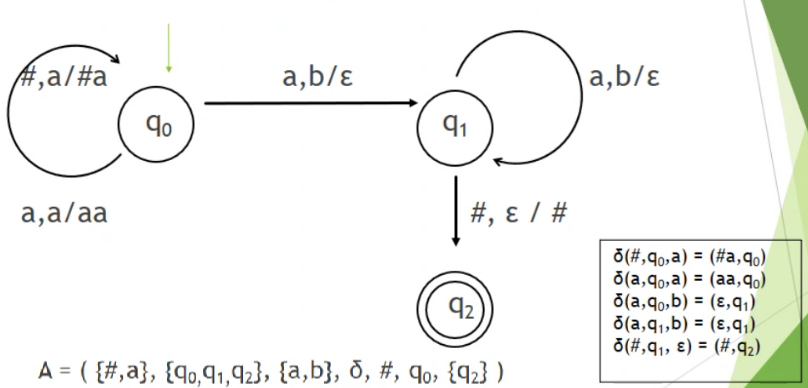
\includegraphics[width=0.7\linewidth]{veremautomata-példa}
\end{figure}

\end{document}
